\section{Results}
\subsection{Modeling Bayes Formula}
\subsubsection{Choosing the Time Limit of Predictions}
On first glance, the most important thing to calculate was the $k$ value, which represented at what time in the future we need to see what is the most probable node that the player is. This value is very important to calculate due to the fact that this constant limits the amount of distance that the PacMan can travel. For convenience issue, we chose this value in the interval $1 \le k \le r$, with $r$ the minimum amount of moves that the ghost needs to reach the player in his actual position. It is important to highlight, that for bigger values of $r$ the prediction is going to be better but, it costs efficiency to the algorithm; on the other hand, this value does not have any limit as, theoretically speaking, the player could go right and left infinite times staying in the same place.

So, the considerations made for this value are to prioritize efficiency at running the algorithm and, this value allows to have a good guess about the optimal move.

\subsubsection{Modeling the Likelihood Distribution}
Now that $k$ has some boundaries, it is important to find all the distributions to calculate this probability. To make this, the game was played by 6 people and recollected data of given a arbitrary position how many times did he move without backtracking. For instance, we count how many moves he made to that place without backtracking; so, if he moved to the right $k-1$ times and to the left the move that was remaining, we considered as a $k-1$ move and so forth. We recollected data from 87 moves with $k$ fixed to the value of 5 and the data recollected can be found in Figure \ref{img:data}.

	  \begin{figure}[H]
          \centering
          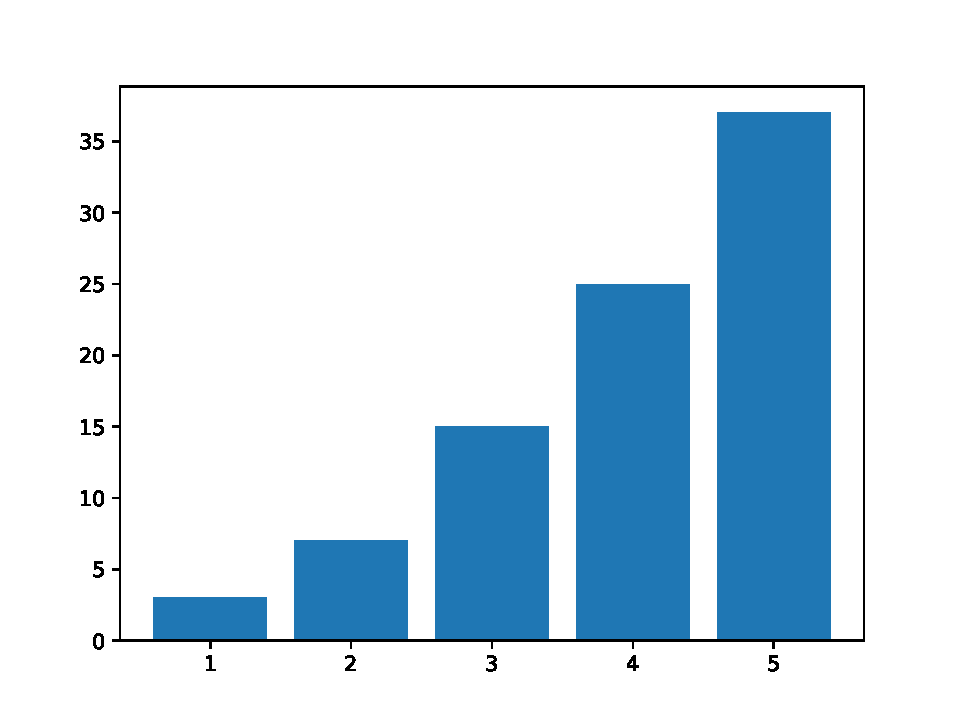
\includegraphics[scale=0.5]{files/Figure_1.pdf}
          \caption{Data recollected of moves of pacman.}
          \label{img:data}
      \end{figure}
      
In this manner, we found that more often than not the player does not back track the move he already made. This is due to the fact that, generally, the player is trying to advance to finish the level by eating all of the points in the map; at the same time, they backtracked only where they were surrounded by ghosts or, they are in vulnerable mode, which leads to take uncommon routes just to kill the enemies.

In conclusion of all of the above, we found that the probability is proportional to the number of movements that the player makes without backtracking to reach that place. Hence, this can be associated to the model of the probability in which node is the player in given a point where this is. Therefore, with this finding we obtain our probability density model for the ${ P }_{ t }=p\wedge { V }_{ t}=v\mid{ N }_{ t+k }$, which is (with $b$ as the number of backtracks the player makes to get to that node respect to the position p):
	\begin{equation*}
      P({ P }_{ t }=p\wedge { V }_{ t}=v\mid{ N }_{ t+k }=n) \quad \alpha \quad (k - b)^2
  \end{equation*}
  \begin{equation*}
      P({ P }_{ t }=p\wedge { V }_{ t}=v\mid{ N }_{ t+k }=n) = \frac {(k - b)^2}{C}
  \end{equation*}

It is important to stand out that $k$ can be calculated as the Manhattan distance from the ghost to the player. Finding $C$ such that this is a probability function, we conclude that the model of the prior distribution is given by:

\begin{equation}
	P({ P }_{ t }=p\wedge { V }_{ t}=v\mid{ N }_{ t+k }=n) = \frac{6(k-b)^2}{k(2k^2 + 3k +1)}, \quad 0 \le b \le k-1
\end{equation}

This equation found is very convenient, although it doesn't represent fully the graph we found in figure 3. On the other hand, we don't need full precision to calculate this probability as, in the long run, we only need to compare which is bigger to decide the movement of the ghost; on the other hand, it would be more appropriate to suppose that this probability is proportional to a power of $k$ for more precision and move the value of the power till finding the exact graph but, we leave it as a suggestion for future work. In this manner, we find that the model found (see the model's graph in Figure \ref{img:real}) is a good approximation of the real model and, it's useful enough for the purpose that it has. 

On the other hand, it is important to emphasize that the likelihood distribution also depends of the velocity of the player but, our model doesn't include this variable. In this manner, we couldn't find a direct correlation between the velocity that the player has and it's relationship to the node; at the same time, this variable is fundamental for calculating later probabilities and for the model to work. 
	\begin{figure}[H]
          \centering
          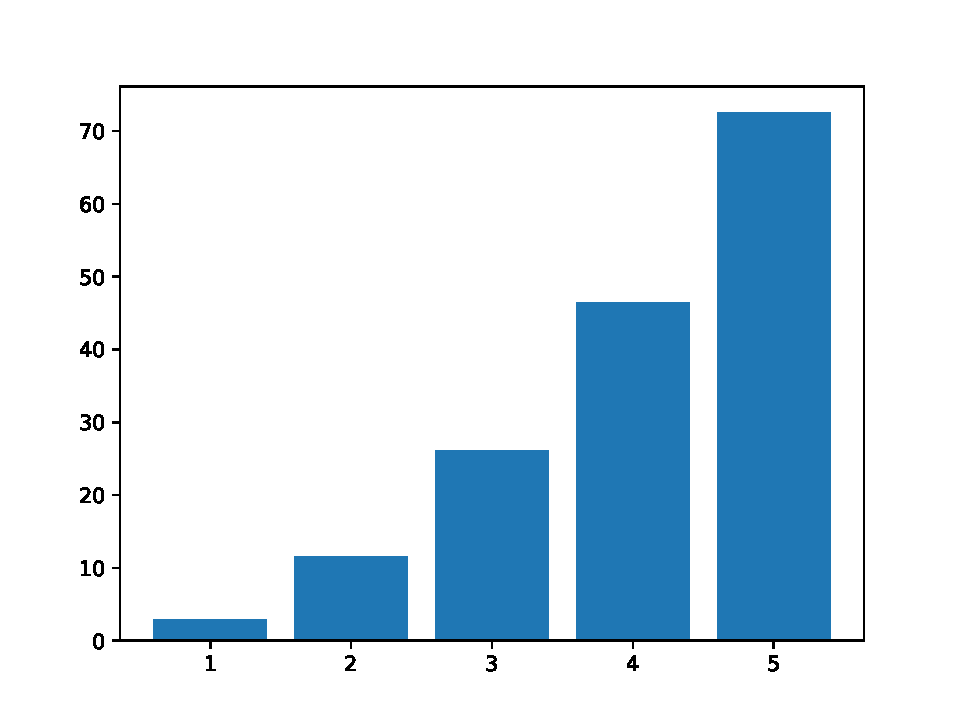
\includegraphics[scale=0.5]{files/Modelo_Teorico.pdf}
          \caption{The same data simulated know by the model found in equation 9.}
          \label{img:real}
      \end{figure}
      
To conclude, it's important to mention that for finding this model it required a lot of peaking and tweaking for making it match the data. In this manner, Bayesian Analysis is a great tool specially for modeling markov chains behavior in video game characters; but, it is difficult to build models to improve the difficulty of the enemies. For future work, we suggest developing tables as seen in the reference \cite{coue2003using} for handling behavior in a easier manner.


\subsubsection{Modeling the Normalizing Term}
As it has already been said, the events of the enemy being in a point $P_t=p$ at a time $t$ and it having a velocity $V_t=v$ are going to be considered as independent events. Therefore, as it was shown in the theory (\ref{subsec:joint}), this normalizing term will be
\begin{equation*}
	P(P_t=p\wedge V_t=v)\,=\,P(P_t=p)P(V_t=v).
\end{equation*}
 Both of the distributions for $P_t$ and $V_t$ will be considered as uniform, since the number of points in the game panel is constant, though it depends on the size of it (which varies depending on the level); on the other hand, there are only 4 possible velocity vectors on each point $p$ at every time $t$, and there is not preference on any of this vectors.
 
Let us define $h$ as the height of the game panel, and $w$ its width; therefore, the uniform density for the random variable $P_t$ will be
\begin{equation}
	P\left( P_{t}=p \right)=
    \begin{cases}
    \frac{1}{wh} & [[0,w]]\times[[0,h]] \\ 
    0 & \text{any other case}
    \end{cases}
\end{equation}
Note that a point $p$ is given by a $(x,y)$ coordinate, and [[a,b]] represents the \textbf{discrete} interval from $a$ to $b$, this is $[[a,b]]=\{a,\,a+1,\,a+2,...,\,b-1,\,b\}$ with $a,\,b\in\mathbb{Z}$. It can be proved that this is, effectively, a density function.

On the other hand, the density function for the velocity vectors will be
\begin{equation}
	P\left( V_{t}=v \right)=
    \begin{cases}
    \frac{1}{4} &  v\in\{(velX,0),(0,velY),(0,-velY),(-velX,0)\}\\ 
    0 & \text{any other case}
    \end{cases}
\end{equation}
As it was discussed in the contributions, the vector can only have one component at a time $t$; it is obvious that this is a density function.

\subsubsection{Modeling the Prior Distribution}
Just as the normalizing factor's marginal distributions, the prior distribution $P(N_{t+k}=n)$ will be a uniformly distributed, since the probability of the player being in any node at a time $t+k$ is the same for all nodes, there will not be preferences for any areas in the game layout. Hence, the density function for $P(N_{t+k}=n)$ is

\begin{equation}
	P\left( N_{t+k}=n \right)=
    \begin{cases}
    \frac{1}{M} &  n\in[[0,M]]\\ 
    0 & \text{any other case}
    \end{cases}
\end{equation}
Where $M$ is total amount of nodes in the games' layout.

Taking all of the above, we end with a posterior distribution:

\begin{equation}
P({ N }_{ t+k }=n\mid { P }_{ t }=p\wedge { V }_{ t}=v)=\frac{24wh(k-b)^2}{Mk(2k^2 + 3k-1)}
\end{equation}

\subsection{Results: Bayesian Inference vs Graph Method}
The algorithm for applying this formula is straightforward. First, as the level starts it sets all the parameters that the distribution needs to calculate the probability; on second place, we set a random node to every ghost so each of them has a different distance from the player; on third place, when the ghost reaches that random node it calculates it's distance to the player and runs an algorithm that finds all of the nodes at a Manhattan distance \cite{manhattan} less tan $k$; finally, it searches for the node with the biggest probability that the player is going to be, and finally moves there.

Although the opposite was thought, the game ran smoothly, even computing bayesian inference constantly. For our tests, the game was played 20 times with the old algorithm (graphs) and the time until the first loss was reported; on the other hand, it was played 40 times after having deployed the new approach (bayesian inference) and, as well, the time until the first defeat was reported. Note that the game with bayesian inference was played slightly more times since it was important to corroborate the proper performance of the ghosts in game and prove that, indeed, they can defeat the player more easily.

This time results are summarized in Table \ref{tab:timeresults}, using common mean calculation, the maximum and the minimum of the data collected; and the complete data for both before and after the model proposed was deployed, is shown in Figure \ref{img:timeresults}.
\begin{table}[H]
\centering
\caption{Game time results before and after the algorithm was deployed.}
\label{tab:timeresults}
\begin{tabular}{ccc}
\hline
\textbf{Quantity} & \textbf{Graph Approach} & \textbf{Bayesian Approach} \\ \hline
\textbf{Mean}     & 24.77                   & 14.75                      \\
\textbf{Max}      & 28.01                   & 20.09                      \\
\textbf{Min}      & 23.56                   & 14.75                     \\ \hline
\end{tabular}
\end{table}
\begin{figure}[H]
  \centering
  \begin{subfigure}[H]{0.4\textwidth}
    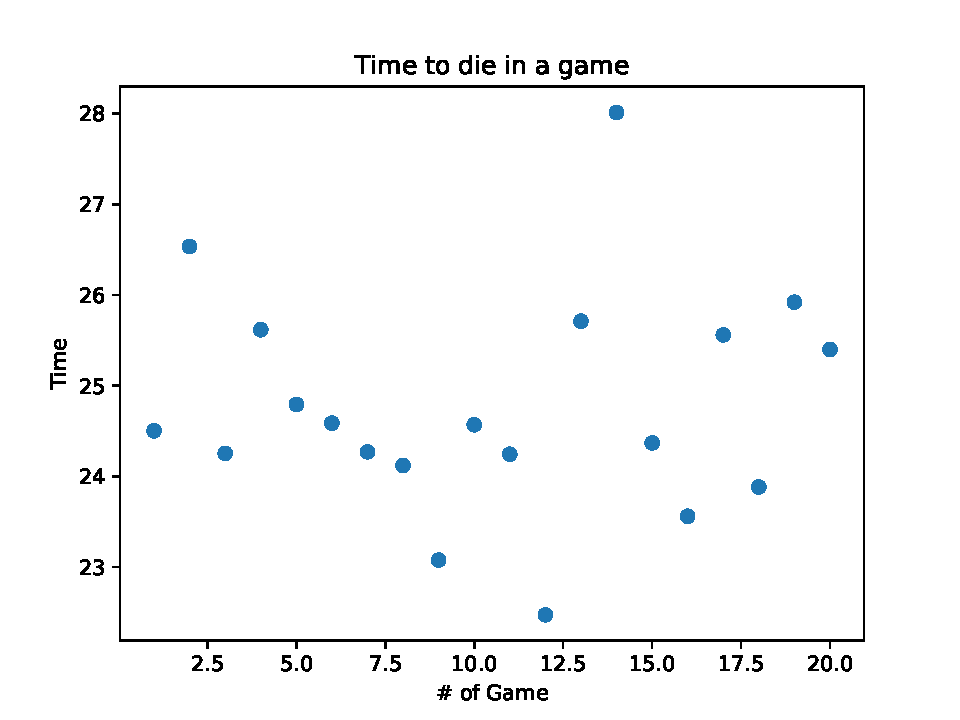
\includegraphics[scale = 0.5]{files/CodigoViejo.pdf}
    \centering
    \caption{Results using graph approach.}
  \end{subfigure}
  \hspace{1cm}
  \begin{subfigure}[H]{0.4\textwidth}
    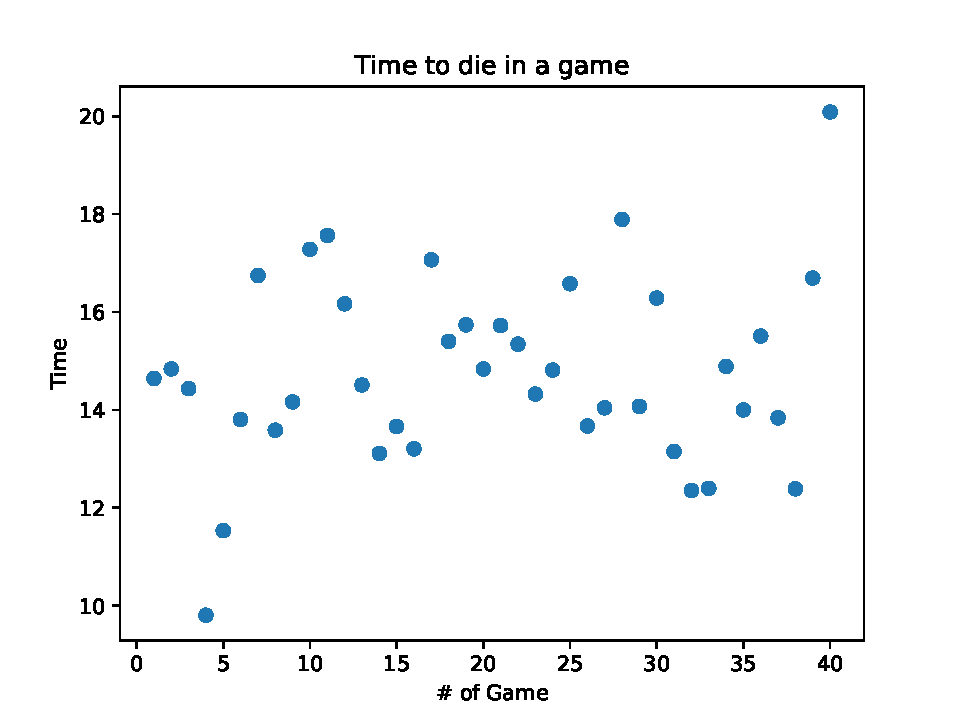
\includegraphics[scale = 0.5]{files/CodigoNuevo.pdf}
    \centering
    \caption{Results using bayesian approach.}
  \end{subfigure}
  \caption{Time until defeat in PacMan.}
  \label{img:timeresults}
\end{figure}

As it is shown in the previous figures, we can affirm that the algorithm is achieving its goals: making a slightly harder gameplay, trying to predict where the player will be and making the overall experience more challenging.












